\documentclass[11pt]{scrartcl} % justified tufte-handout
%Gummi|065|=)
\title{\bfseries Differentiable Trajectory Optimization\\ Under Uncertainty}


%\usepackage{classico}
\usepackage{microtype}
\author{Joan Creus-Costa\and John Dean}
%\date{}
\usepackage{amsmath}
\usepackage{amssymb}
\usepackage{graphicx}
\usepackage{wrapfig}
\usepackage{xcolor}
\begin{document}

\maketitle

\def\States{\mathcal{S}}
\def\Altitudes{\mathcal{H}}
\def\Velocities{\mathcal{V}}
\def\Lifts{\mathcal{L}}
\newcommand{\mx}[2]{\left[ \begin{array}{#1} #2 \end{array} \right]}

\tableofcontents

\section*{Nomenclature}
\begin{tabular}{rl}
$h$ & altitude  \\
$v$ & vertical velocity\\
$\ell$ & net lift \\
$w_{\dot \ell}$ & disturbance on lift \\
$w_{v}$ & disturbance on the vertical velocity of the balloon (wind) \\
\end{tabular}

\section{Altitude control}
\subsection{System dynamics}

High Altitude Balloons utilize a lifting gas that is lighter than air to produce a buoyant force to counteract the force of gravity on the balloon membrane and the payload. The buoyant force on the balloon minus the force of gravity on the balloon is refereed to as net lift, $\ell$. ValBal uses a valve system to vent lifting gas and a ballast system to drop small mass pellets, to change the net lift of the balloon. This net lift produces an acceleration on the system, causing the balloon to accelerate upwards or downwards until the force of drag on the system equals the net lift, at terminal velocity. Because the balloon accelerates to terminal velocity quickly after a change in net lift, the balloon's vertical velocity, $v$, can be approximately modeled as always traveling at terminal velocity.

While the force of drag on the balloon is nonlinear with respect to velocity, for the purposed of modeling and control, it can be linearized within a range of reasonable velocities. After doing so, the system dynamics can be simplified to:

\[ v(t) = k_d \ell \qquad \dot h(t) = v(t)\]

With $k_d$ being the linearized coefficient relating net lift to velocity. The valve and ballast system of can be seen as changes to the derivative of the net lift of the balloon, $\dot \ell$. For example, when the valve is open, $\dot \ell$ becomes negative as the balloon looses lift. In addition, the atmosphere is full of disturbances, so in the system dynamics we consider 2 other terms: $w_{\dot \ell}$ as the atmospheric disturbance on the lift rate, and $w_v$, as the atmospheric disturbance of velocity. For example, at night the balloon cools and looses lift, which is modeled as a negative $w_{\dot \ell}$, and vertical winds are modeled as a nonzero $w_v$. With these additions, the system dynamics become

\[ \dot v(t) = k_d(\dot \ell(t) + w_{\dot \ell}(t)) \qquad \dot h(t) = v(t) + w_v(t) \]

Using the following substitution we can write the a state-space representation of the system. 

\[x = \mx{c}{h \\ v} \qquad u = \dot \ell\]
\[\dot x = \mx{cc}{0 & 1 \\ 0 & 0}x + \mx{cc}{0 \\ k_d} u + \mx{c}{w_v \\ k_d w_{\dot \ell}}\]

\subsection{Control system}


\subsubitem{Simulations}


\begin{figure}[h]
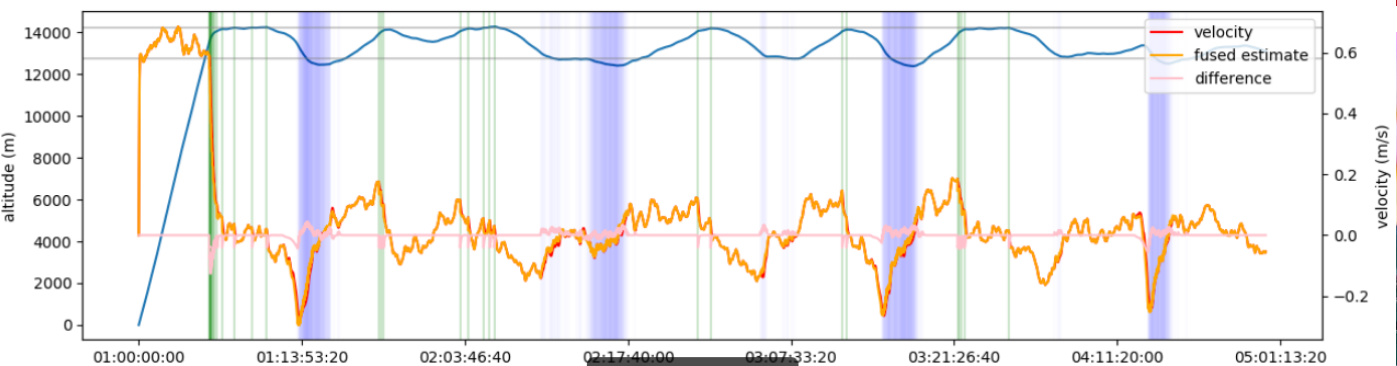
\includegraphics[width=1\linewidth]{lsim.png}
\label{lsim}
\end{figure}


\newpage
\section{Trajectory planning}
\subsection{Introduction}

ValBal has no direct control over it's lateral movement around the globe, but rather is always drifting with the air currents of earth's atmosphere. However, by changing the altitude that it flies at, it can choose different wind currents moving in a range of directions in a given column of air. The high-level goal of trajectory planning is to come up with these altitudes that the balloon should fly at in order to achieve some mission outcome in the lateral trajectory of the balloon.

[Literature review]



\subsection{Formulation}
The physical system is represented by continuous states $s\in\States$ defined at discrete times $t_k=t_s + k \Delta t$, for $k=0,1,\dots$ In the case of ValBal, we can let $\States=\Altitudes\times\Lambda\times\Phi$, if we're considering altitudes, latitudes, and longitudes; we could extend this to include the ballast levels $\mathcal{B}$, or lifts $\Lifts$.
% This might want to go in an introduction subsection
The altitude changes with respect to time according to the setpoint altitudes given to the control algorithm, with some randomness due to atmospheric noise. Latitude and longitude change according to Euler integration of the wind field, evaluated at every given time, altitude, and coordinates. Our goal is to find a policy to maximize some objection function, which might, for instance, be the total horizontal distance travelled.

While traditional methods of finding a policy to optimize a physical system rely on discretizing the state space, we note that this is highly intractable to do in this situation, for various reasons:
\begin{itemize}
\item The state space is extremely large, even if we restrict ourselves to the bare minimum and discretize coarsely. Methods such as policy iteration would likely take unbearably long.
\item The underlying dynamics are continuous, and in fact very easy to integrate. If we discretize the state space, we would lose resolution in the integration. Furthermore, the noise between discretized time steps is correlated; therefore, unless we take very large time steps, or increase the size of the state space, the Markov assumption will not hold, and the policy will not properly handle uncertainty.
\end{itemize}
While clearly keeping the state space continuous (only discretizing time) makes integration a lot easier, it makes finding a policy harder: the optimal policy is highly nonlinear due to the characteristics of atmospheric wind patterns, and our desired map $(t,h,\phi,\lambda)\to (h_s, \Delta_s)$ (from time, altitude, and coordinates, to a setpoint altitude and a tolerance around it) is high dimensional. A key realization is that, while the map is highly nonlinear, it is generally smooth, and doesn't have many local minima: wind patterns are generally spatially large and temporally slow moving.

This results in another advantage that comes from keeping the state space continuous. By picking some fixed set of parameters $\theta$ (that might be the setpoint altitudes and tolerances at various points of the flight) and integrating the trajectory as a function of those parameters, we can take the gradient of the cost function (that is a function of the trajectory) with respect to the parameters, and optimize our objective. We expand upon a formulation in the following section.

\subsubsection{Differentiable altitude trajectory}
Ultimately, our goal is to come up with some continuous and differentiable function $V(\theta)$ that gives the value of the objective function. However, in many instances, the value of the objective function will be related to the integration of the trajectory---e.g. distance travelled, or final longitude. This means that we need to come up with a formulation of the trajectory that depends on the optimization parameters and is differentiable with respect to them.

The parameters that form $\theta$ can, for instance, be a set of altitude waypoints defined at various points of the flight, or altitude tolerances at each of those points. If our state consisted only of altitudes, and we were to simply linearly interpolate between altitude waypoints $\theta_0, \theta_1, \dots$ (defined at $t^w_0, t^w_1, \dots$) we would find the parameters relevant to the current timestep $t_k$ such that $t^w_i < t_k < t^w_{i+1}$. Then we simply give:
\[h(t_k; \theta) = \theta_i + (t_k - t_i^w) \frac{\theta_{i+1}-\theta_i}{t_{i+1}^w - t^w_i}\]
which has a very simple derivative with respect to the optimization variables $\theta$. However, this assumes that we follow \emph{exactly} the trajectory defined by the optimization parameters. In reality, the value function $V(\theta)$ will be taken over an expectation ensemble of possible trajectories under noise.

In other words, our trajectory integration needs to output a distribution of possible states it might end up, while remaining differentiable. We introduce a parameter $\lambda$ that can be interpreted as a percentile of the noise distribution that a given trajectory is under. At the beginning of a rollout, a sequence $\lambda_0, \lambda_1, \dots$ is randomly generated such that the variation results in a noise level consistent with flight data. In the limit where all $\lambda$ are 0.5, the median trajectory is selected; in a more realistic simulation, the percentile would slowly fluctuate between smaller and larger numbers such that a particular rollout would be flying low or high respectively with respect to a noise-free simulation. For instance, in the scenario given above, we could introduce $\lambda(t)$ as a random walk bounded between $-500~\textrm{m}$ and $500~\textrm{m}$, defined between $t_0$ and $t_f$. Then our position is given by:
\[h(t_k; \theta) = \theta_i + (t_k - t_i^w) \frac{\theta_{i+1}-\theta_i}{t_{i+1}^w - t^w_i} + \lambda(t_k)\]
This allows us to consider a stochastic evaluation of our value function that remains differentiable.
\[\tilde V(\theta)=\sum_{\textrm{random}~\lambda} F(t_f, \lambda; \theta)\]

\subsubsection{Differentiable horizontal trajectory} \label{sec:horizontal}
The section above only handled altitude; however, the objective function for ValBal relies on maximizing spatial parameters, and not altitude. The horizontal integration needs to preserve differentiability to be able to compute a full gradient with respect to every optimization parameter. We use atmospheric data provided by \textsc{noaa} which, in particular, includes the velocity field $w(h, \lambda, \phi, t)\to(u, v)$, where $h$ is the altitude defined on a set of forecast altitudes;\footnote{The data from \textsc{noaa} is defined at barometric pressures, which can be mapped monotonically to altitude.} $\lambda$ and $\phi$ are the coordinates defined on a (not necessarily regular) grid of latitudes and longitudes;\footnote{Some models are more regular than others; for instance, NAM is defined on a rather annoying Lambert conformal grid.} $t$ is a forecast time (usually separated by 1 to 3 hours) and $(u, v)$ are the two horizontal components of wind.

For completely regular grids, bilinear interpolation will suffice. For irregular grids, a scheme such interpolation weighted by inverse distance $(\sum^K \alpha_i w_i)/(\sum^K \alpha_i)$ for the closest $K$ points would do the job. The weights of each nearby point are a function of altitude, latitude, and longitude; therefore, when we take the weighted sum, we preserve a differentiability path through the (differentiable) altitude. In other words, the final velocities $(u_k, v_k)$ are themselves a function of $\theta$, which we use to find the new coordinates:
\[x_{k+1} = x_k + u_k\Delta t\quad y_{k+1} = y_k + v_k\Delta t\]
and the conversion to $(\lambda_k, \phi_k)$ follows from a simple computation of spherical coordinates. 

The viability of this method, as well as the quality of \textsc{noaa} data can demonstrated by comparing the integration method and wind model to previous balloon flight data.

{\color{red} Words to go here}

\begin{figure}[h]
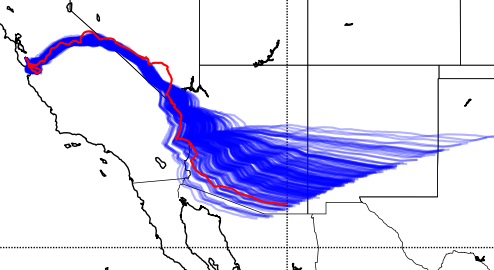
\includegraphics[width=0.5\linewidth]{winds.png}
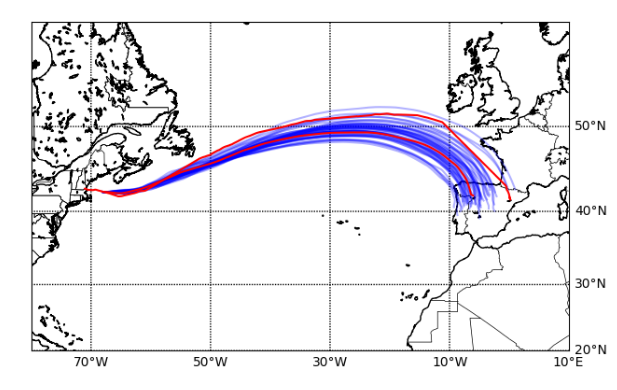
\includegraphics[width=0.5\linewidth]{spain.png}
\label{winds}
\end{figure}

\subsubsection{Differentiable value function}
We can consider a variety of value functions. If we're trying to maximize the horizontal function, we can use the differentiable longitude computed in Section~\ref{sec:horizontal}. For a rollout of length $K$, the total value is the horizontal distance:
\begin{equation}
V = \sum_{k=0}^{K-1} u_k \Delta t\label{eqn:value}
\end{equation}
where $\Delta t$ is a constant that does not affect the result. Other valid objective functions could include the distance to a particular point:
\[V = \sum_{k=0}^{K-1} \lVert r_k - r_\text{target}\rVert\]

\newpage
\subsection{Preliminary Results}
\subsubsection*{Certainty Equivalent}
Before running the full stochastic gradient decent on the monte-carlo problem, we developed and tested the algorithm on certainty-equivalent simulation with no noise. In this experiment, we optimized a single starting trajectory, assuming that we had complete control over 20 altitude way points, with the balloon linearly interpolating between them. The results of such a test are shown in figure \ref{ce}. 

\begin{wrapfigure}{l}{0.5\textwidth}
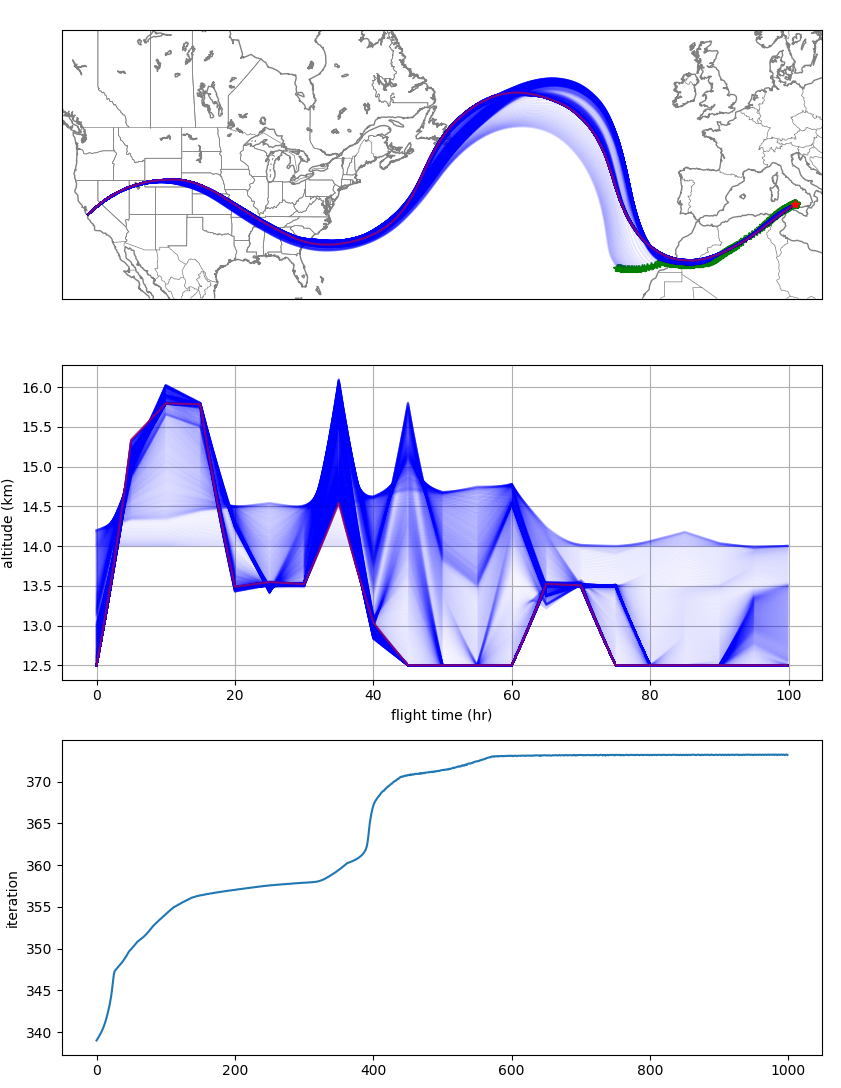
\includegraphics[width=1\linewidth]{certaintyeq.png}
\caption{Certainty equivalent optimization from a single trajectory of the total longitude traveled. Trajectories are depicted both in latitude vs longitude over a Mercator projection (top), and altitude vs time (middle). The launch site simulated was Hollister, California and flight endpoints are designated with a green star. Intermediate trajectories are show in blue, with the final optimized result in red. A convergence plot of the objective function vs iteration number is shown (bottom)}
\label{ce}
\end{wrapfigure}

We can see from this figure, that the optimization behaves as expected. The final longitude slowly moves forward each iteration, until it is at reaches a local extremum. The path of green points over the map--the endpoints of each intermediate trajectory, always moves to the right as iteration number increases.  Running the 1000 iterations of certainty equivalent optimization on a 100 hour flight such as this take well under a second on our hardware.


\subsubsection*{Monte-Carlo}

To run our first test of this formulation, we we opted to utilize the traditional Model Predictive Control approach, in which we optimize an open-loop policy over a finite horizon. In flight, this optimization would be ran again and again as the balloon flies, using the most recently observed system state to optimize new trajectories, forming a feedback control law. 

Results of this method on a sample of \textsc{noaa} analysis wind data is show in figure \ref{openloop}.
\begin{figure}[h]
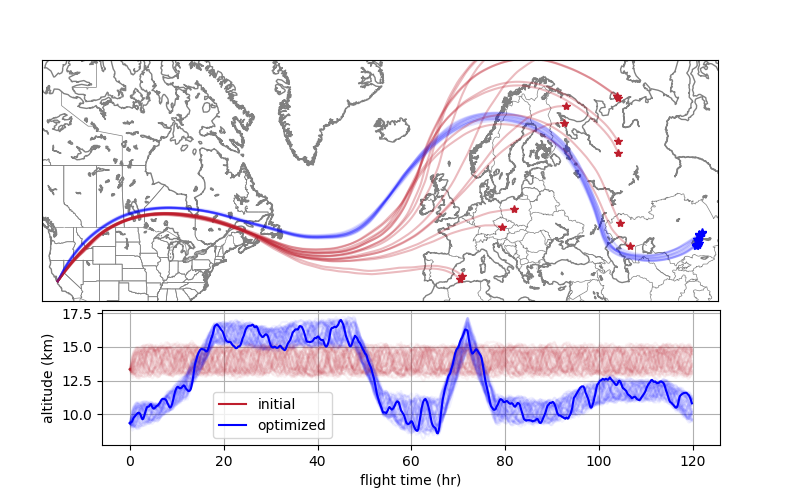
\includegraphics[width=\linewidth]{datasheetfig.png}
\caption{Example result of optimizing an open loop trajectory. The initial settings were a 13.5km setpoint and a 0.75km tolerance (red), while the optimized trajectory shows both changing setpoints and tolerances (blue). The dark blue line gives an example possible altitude profile from the many possible altitudes profiles given the command settings}
\label{openloop}
\end{figure}

We notice a few things from this result. First, that in this particular scenario, the initial commands resulted in a large variation in the resulting flight path. This was due to large changes in wind direction within the command tolerance over the Atlantic ocean. We see that in the optimized open-loop trajectory, policies are picked such that there is not much variation in the resulting outcome. 



\newpage
\section{Architecture}
In this section we describe the architecture behind the simulations and trajectory optimization. It involves a complex pipeline, that involves fetching atmospheric data, a modular and fast simulation engine, and provisions for simulating with real flight code. It is mostly written more than two thousand lines of C++ and Python.

The core of the simulator is written in C++. This allows for extremely fast simulations; when performing direct rollouts, it can compute hundreds of thousands of three-day ValBal trajectories per second on a 6-core machine. The code is designed to be modular; one can easily use different objective functions (horizontal distance, distance to a given target\dots), different optimization methods (vanilla gradient descent, Adagrad, Adam\dots), various differentiable controllers (uniform distribution, approximate Lasagna, differentiable Lasagna\dots), and so on.

Having been designed with optimization in mind, another key feature of the simulation codebase is the formulation in terms of C++ templates, that allow the compiler to, from a single codebase, generate code that either merely computes rollouts of the trajectories, or keeps track of the gradients leading to the final objective function. The latter uses \emph{automatic differentation}, the same algorithm used in the training of large neural networks. It keeps track of the computation graph and derivative at each node; once the final objective function is computed (say, the final longitude), the gradient is propagated backwards to each parameter, and some first-order optimization method is used to update the parameters. By using the Adept library, the parametrized codebase can be specialized to use Adept's differentiable floating point type, that keeps track of the computation graph. Doing so incurs an overhead, of about 5 to 10$\times$, but is able to provide the exact gradient of the objective with respect to the parameters, in a much easier way than direct numeric differentiation, and without having separate code paths for direct evaluation and gradient evaluation.

We also built several Python scripts to fetch the data and process the results. We can retrieve wind data from either the Global Forecast System (\textsc{gfs}) model from \textsc{noaa}, or the European \textsc{ecmwf} model. We preprocess the data, that comes in \textsc{grib} files, into binary files that are loaded directly by C++. This is key to the speed of the C++ codebase, by using the \texttt{mmap} system call from Linux, the data will end up cached in the comparatively faster RAM, and wind table lookups require merely the computation of an offset (as opposed to searching through a database, with various levels of indirection). In particular, we only store relevant variables at the altitudes ValBal normally flies, in order to save space and improve cache performance. Several Python scripts are used to plot the trajectories found by the C++ script (saved to a binary file) using the Matplotlib library.


\section{Flight Test}




\end{document}
